\chapter{Discussion}

\section{The Big Picture}\label{sec:bigpic}

In Chapter~\ref{chap:morph} I discussed how the results presented suggested that quenching rates with $\tau < 1.5~\rm{Gyr}$ must be caused by mechanisms which can transform morphology from spiral to elliptical. This does not infer an immediate switch from disc dominate to elliptical however. Indeed work by the \textsc{ATLAS}$^{\rm{3D}}$ team showed that kinematic dissks are found int he majority of the visually elliptical population \citep{citationbomb} with $\sim2-5$ times the number of \emph{fast rotators} with kinematic discs than \emph{slow rotators} with dispersing dominated kinematics. 

The results of these works suggest that major mergers which can destroy the disk dominated nature of a galaxy \citep{refs} in rapid timescales may produce last rotators. I find across the red sequence population in Figure~\ref{red_s} that $6\%$ of the population density lies below $\tau <0.1 \rm{Gyr}$, in agreement with predictions that $7\%$ of ellipticals are indeed slow rotators \citep{refs}. This therefore provides an estimate for the percentage of the galaxy population whose histories are dominated by dry major mergers.  Conversely fast rotators could be formed by the slow build up of a galaxy's bulge over time, until it eventually swallows the disc. This growth is thought to occur via interactions, wet major and minor mergers and disc instabilities which can produce a visually elliptical, quenched galaxy residing on the red sequence. Previously, major mergers were considered the only mechanism which could achieve such a result, however I speculated in Chapter~\ref{chap:morph} that all mechanisms with $\tau < 1.5 ~\rm{Gyr}$ can cause a morphological change mid-quench. This gradual, slower evolutionary history explains why studies have concurrently found that the major merger rate is muuch lower than expected given the observed red sequence ($\sim 10\%$,  ?$\%$ lower than expected \citealt{refs}). Larger IFU studies of MaNGA, SAMI and CALIFA will allow for larger populations of slow and fast rotators to be identified so that the relative dominance of wet and dry mergers across the elliptical population can be determined more accurately. 

A property which I have also overlooked in this work, but which is often investigated in quenching studies is the stellar mass surface density of a galaxy, alternatively the ``concentration'' of a galaxy, which is found to correlate with the SFR of a galaxy. The build up of a galaxy's bulge is thought to be able to stabilise a disk against collapse and effectively stop it from forming stars. This is classed as a type of morphological quenching and is effective over $\sim\rm{Gyr}$ even if gas is still externally fed to a galaxy. This slower quenching track of bulge dominated galaxies may help to explain the slow quenching rates observed across the red and green smooth weighted population densities seen in Figures~\ref{red_s} \& \ref{green_v}, which suggest that this may be occurring in up to $40\%$ of the smooth weighted population (see Figure~\ref{red_s}). By observing the population densities in these figures we can separate the processes which both quench and grow the bulge simultaneously and those which only grow the bulge and quenching is consequently achieved slowly by morphological quenching. However, even in the former case, morphological quenching may help in either speeding up the process or in keeping the galaxy quenched post interaction. This is supported by the finding of \cite{abramson16} who found there is no threshold at which density triggered quenching occurs, but that deer systems typically redden faster than less dense galaxies. This one again suggests a continuous nature of processes affecting galaxies across their lifetimes, as discussed in Chapter~\ref{chap:env}, suggesting a symbiotic partnership between minor mergers and morphological quenching to achieve true quiescence. 

This is similar to the idea discussed in Chapters~\ref{chap:morph} \& \ref{chap:agn} that without AGN feedback a major merger cannot fully quench a galaxy. A shown in Figure~\ref{rate}, an AGN doesn't always cause quenching at the rapid rates suggested by major mergers, but that a slow co-evolution of black hole and host galaxy can occur. Left alone, AGN are only efficient as a quenching mechanism in low mass galaxies where they can have a greater impact. In combination with a major merger however, they can have catastrophic effects. These effects are therefore easily detectable, leading to the initial theories for the widespread links between AGN and mergers \citep{refs bomb}. However, by styling the population as a whole with more robust statistics, the more subtle role of AGN across the population is revealed. 

The resulted throughout Chapters~\ref{chap:morph}-\ref{chap:env} have revealed the interplay between all of the mechanisms proposed in Chapter~\ref{chap:intro}, including different environmentally driven mechanisms, mergers \& AGN, disc instabilities \& the environment and minor mergers \& morphological quenching. All of these mechanisms are striving towards the same env goal of galaxy quiescence with no single mechanism dominating over another, except in the most extreme environments or mass. While mass and morphological quenching will be far more likely to occur in the field, they still impact galaxies in the densest environments. Similarly, mergers will be far more likely to be a part of a galaxy's evolutionary history if it resides in dense environments and will often drown out the more subtle effects of slower quenching mechanisms at work before the merger occurred. 

The dominance of each mechanism is therefore a matter of circumstance. Just as galaxy morphology is a spectrum of trucker from the most disc dominated to the most spheroid dominated systems so too are the quenching mechanisms which can cause this change. Mergers are a spectrum of mass ratios from micro mergers \citep{carlin16} through to major mergers, which have increasingly devastating impact upon the morphology and SFR of a galaxy. Morphological quenching mechanism,s lie on a spectrum of mass and stellar mass surface density, whereas environmentally driven quenching mechanism lie on a spectrum of increasing halo mass. All of these mechanisms, depending on a galaxy's environment are likely to affect a galaxy at some point in its lifetime, working in collaboration to reduce the SFR over a continuum of timescales. Rather than focusing on isolating the effects of a single  dominant mechanism, future galaxy evolution studies should attempt to understand the interplay of all possible quenching mechanisms over cosmic time. 

\section{The use of morphology in large surveys}\label{sec:usemorph}

As discussed in Section~\ref{sec:bigpic}, I like to consider morphology as a continuous spectrum from disc dominated to bulge dominated systems roughly reflecting the continuous nature if galaxy evolution. This continuous nature is reflected by the parameters use to characterise the structure of a galaxy, including S\'ersic index \citep{ref}, Gini coefficient \citep{ref}, asymmetry \citep{ref} and concentration index \citep{ref}. the problem arises when studies discretise this back to the typical distinct Hubble classifications of morphology \citep{citationbomb}; either the data is mapped to T-types \citep{refs} or merely split bimodally into late and early types, with e.g. $n \leq 2.5$ to identify discs \citep{refs}. This tendency to split populations bimodally is a common trope across the astrophysical community. Although this classification is physically motivated in some cases, such as Cephid variables and planet classification, in other instances this is not the case, e.g. Type 1 and 2 Seyferts, slow and fast rotators, slow and fast rotators, long and short gamma ray bursts and supernova classifications. 

For large surveys where a large amount of effort is placed in multi-component fitting \citep{refs} the use of morphology is particularly important as we must understand how to effectively utilise these fits hen studying the effects of morphology. It is unsurprising that previous studies of galaxy evolution while split the galaxy population bimodally into early- and late-types galaxies have concluded there are two dominant evolutionary histories \citep[e.g.][]{schawinski14}. However, I have shown that this is not the case, finding a continuous distribution of quenching rates across the galaxy population. I believe that this result is possible (in part due to the robust statistical method employed) due to the correct use of the full data set which is weighted by the continuous GZ vote fraction estimating the likelihood of either a disc or smooth galaxy. Adapting such methods in future studies will allow the `high hanging fruit' science results to be picked out from both archival data and upcoming large surveys, such as LSST \citep{}. 


\section{Future Work}\label{sec:future}

Due to the flexibility of the \starpy\ package I believe it will have a significant number of future applications. Firstly by investigating quenching using different wavebands as star formation indicators. For example, using the $U-V$ and $V-J$ colours used to separate star forming and quiescent galaxies on the UVJ diagram \citep{ref} at higher redshift (out to $z\sim4$) in the COSMOS/ULTRAVista fields \citep[e.g. see work by][]{muzzin13} will help to further constrain the relative interplay of quenching mechanisms across the galaxy population with cosmic time. Morphologies are also available for the COSMOS field with the recent release of the \textsc{gz:hubble} classifications in \cite{willett16}. Secondly, by expanding the possible SFHs which can be assumed for a galaxy, \starpy\ could be expanded to use Bayesian evidence to chose which is the most appropriate history to characterise the photometry. The currently exponentially declining SFH (the so called ``$\tau$-model") used is considered the simplest possible SFH one can assume and so more detail about he effects of different quenching mechanisms may be elucidated by increasing the complexity. For example, possible SFHs include a starburst model \citep{ref}, adding a third variable for time of galaxy formation \citep{ref}, a Gaussian increase in the SFR, rather than a constant value before $t_q$ or a log-normal SFR \citep{gladders13, abramson16}. 

Along with this expansion of the \starpy\ module itself, several avenues of data exploration are still available using \starpy:
\begin{enumerate}[(i)]
\item A comparison of a large population of fast and slow rotators; this would aid in the understanding of the different quenching timescales of wet and dry major mergers. 
\item A study of barred vs non-barred galaxies using $\{p_{\rm{bar}}, p_{\rm{no bar}}\}$ in place of $\{p_{\rm{disc}}, p_{\rm{smooth}}\}$ used to weight the population densities seen in Chapters \ref{chap:morph} \& \ref{chap:agn} may reveal the impact a bar can have on a galaxy's SFR by funnelling gas to central regions.
\item Studying the SFHs of low mass satellite galaxies with $M_* \leq 10^{8-9} ~M_{\odot}$ which may have quenching histories dominated by ram pressure stripping for which the observational timescales are still uncertain. 
\item Expanding the study of the effect of AGN feedback by investigating the SFHs of unobscured Type 1 AGN (however this would require either a more accurate subtraction of the unobscured nuclear emission or a change in the bandpass input to \starpy\ to negate this issue) and those identified with X-ray and IR selection methods. Confirming the result seen in Chapter ~\ref{sec:agnfeedback} with these AGN would coobborate the idea that quenching is occurring across the entire AGN population, and provide further support for the theory of AGN unification \citep{antonucci93, urry95}.
\end{enumerate}

\section{The use of \starpy\ with IFU data}\label{sec:IFU}

In Chapter \ref{chap:agn} I discussed how the current SDSS data (both photometric and spectroscopic) cannot determine whether the AGN is the cause or the consequence of the quenching seen across the AGN host population in Figures \ref{time} \& \ref{rate}. Using data form the MaNGA \citep{bundy15} IFU survey I hope to determine whether the AGN is truly the cause of this quenching via AGN feedback. The MaNGA surgery will provide 127 spectra across a single galaxy (see Figure~\ref{fig:manga}), allowing the SFH to be mapped as a function of radius for the first time. Not only that, but the acquisition of a spectra in each of these apertures allows for the modification of \starpy\ to take spectral star formation indicators \citep[such as $H\alpha$][]{ref} to break the degeneracy provided by the photometric colours (see Figure~\ref{pred}) and the easy removal of any unobscured AGN in the central regions. 

\begin{figure}
\centering{
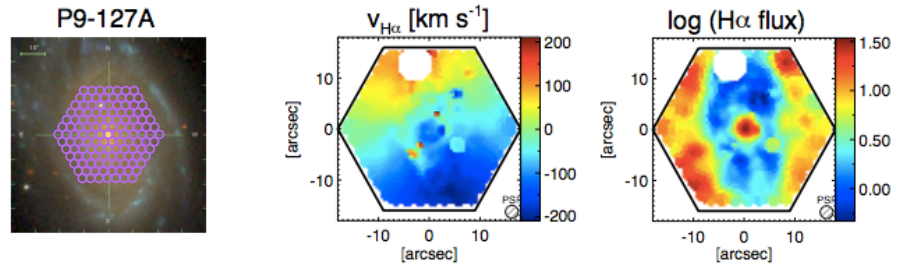
\includegraphics[width=0.95\textwidth]{discussion/manga_data.png}}
\caption[Example MaNGA fibre bundle on a target galaxy with example emission data]{Example fibre bundle placed over a MaNGA target galaxy (left) and corresponding data from the P-MaNGA survey showing the mapped velocity (middle) and flux (right) of $H\alpha$ gas emission as measured across the galaxy in the fibres. Such measurements can be utilised to calculate the star formation rate across the structure of a galaxy. Adapted from \cite{bundy15} Figure 14.}
\label{gal}
\end{figure}

Any correlate of the output quenching parameters with radius of the galaxy will allow the determination of whether quenching is happening from the outside-in \citep[i.e. due to the environment, as in][]{ref, ref} or inside-out, as in initial work by \citet{ref}, and whether this correlates to the presence of an AGN across the galaxy population.

\section{Hubble space telescope follow up}\label{sec:hst}

In Chapter~\ref{chap:agn}, I discussed how accurate fits to the bulge-to-total ratio could not be made for galaxies of the bulgeless sample hosting AGN duet the resolution of ground based SDSS imaging. This led to the derivation of upper limits on the bulge masses of this sample. The Hubble Space Telescope (HST), however provides (a) an extremely stable and well understood point spread function, enabling reliable separation of the active nucleus from its host, and (b) high spatial resolution which is needed to distinguish between classical, merger driven bulges and pseudo bulges. Observations with the HST of the galaxies in the \textsc{bulgeless} sample will enable extremely accurate measure of bulge-to-total ratios for each host galaxy and allow the identification of truly secular systems with growing black holes. Such measurements will also allow the interplay between merger driven (building classical bulges) and merger free (building no or pseudo-bulges) co-evolutionary histories to be disentangled. 

Figure~\ref{fig:hstdata} demonstrates the difference in resolution provided by the HST with one of the first image from proposal 12424? in Cycle 24? of the bulgeless galaxy J$192250.74$-$055259.15$ in comparison with the ground based SDSS ugriz image (also shown in Figure~\ref{fig:INTimages}. This image will allow for the robust derivation of the bulge mass of this galaxy, allowing for a more concrete conclusion to be drawn on the controversial issue of secularly driven galaxy-black hole coevolution. 

\begin{figure}[h]
\centering{
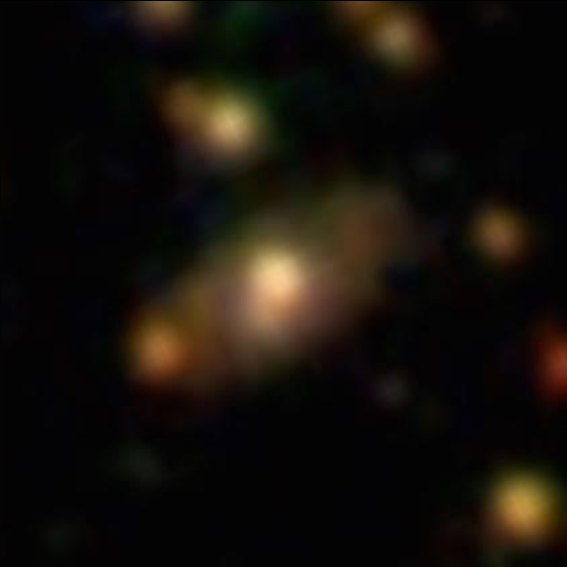
\includegraphics[width=0.49\textwidth]{discussion/sdss_data.png}
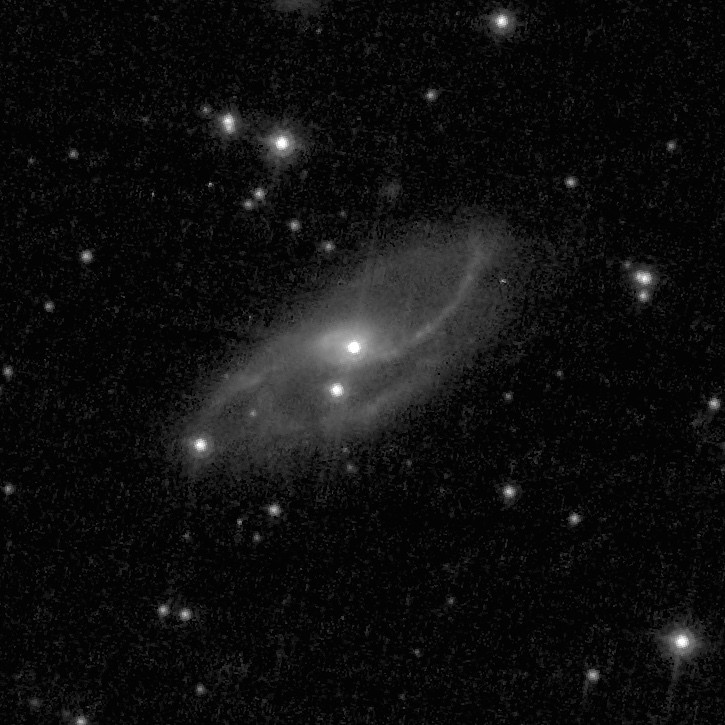
\includegraphics[width=0.49\textwidth]{discussion/hst_data.jpg}}
\caption[Example HST image data in comparison to SDSS]{Example SDSS urgiz image (left) for J$192250.74$-$055259.15$, part of the \textsc{bulgeless} sample, described in Section~\ref{sec:selectAGN}, in comparison to space based imaging from the HST (right). The higher resolution HST image reveals finer structure than the SDSS image and the true disc dominated nature of the galaxy.}
\label{gal}
\end{figure}
